·% !TeX root = ../thuthesis-example.tex

\chapter{实验与分析\label{sec:chap8}}
本章对前文中所提出的优化设计进行实验,验证这些设计的效果。本章首先介绍实验环境,然后验证在客户端将 \emph{insertRecords} 请求转换为 \emph{insertTablets} 请求带来的性能提升,再验证在不能转为 \emph{insertTablets} 请求的场景下各个优化工作对 \emph{insertRecords} 写入带来的性能提升。最后介绍用户负载采样程序和模拟程序,将所有优化点综合在一起,模拟在用户负载下的性能提升。
\section{实验环境}
\begin{table}
  \centering
  \caption{实验环境}
  \begin{tabular}{ll}
    \toprule
    配置名称 & 配置值 \\
    \midrule 
    CPU & I7-11700 8C16T 2.5GHz\\
    内存 & 32G DDR4 3200 Mhz\\
    DataNode 内存 & 28G \\
    ConfigNode 内存 & 2G \\
    机械硬盘 & 希捷 ST-16000NM000J \\
    JDK 版本 & OpenJDK 11.0.22 \\
    操作系统版本 & Ubuntu 20.04.2 LTS,64 位 \\
    网络环境 & 1000 Mbps 局域网 \\
    \bottomrule
  \end{tabular}
  \label{tabular:iotdb-runtime-config}
\end{table}

表 \ref{tabular:iotdb-runtime-config} 展示了测试所用的硬件环境和软件环境。测试机器分为两台,配置均与表格中展示的一致,一台用于运行 IoTDB,另一台则用于运行测试程序。IoTDB 在部署时将一个 DataNode 和一个 ConfigNode 部署到了同一台机器上,DataNode 分配了 28G 的内存,ConfigNode 分配了 2G 的内存。IoTDB 使用了一块希捷 ST-16000NM000J 机械硬盘作为存储设备,系统数据、写前日志、系统运行日志等都会存储在同一块磁盘上。IoTDB 使用了 OpenJDK 11.0.22 作为运行环境,操作系统为 Ubuntu 20.04.2 LTS,64 位。测试机器之间的网络通过 1000 Mbps 的局域网连接。在某些实验中,为了模拟更低的网络带宽,我们使用了 wondershaper 工具限制了网络带宽。

\section{客户端请求格式转换性能试验}
在这一节中,我们测试了在客户端处将 \emph{insertRecords} 请求转换为 \emph{insertTablets} 请求所带来的性能提升。我们使用 IoT Benchmark 作为测试程序,并且将客户端的转换系数设置为 0.5,即只要平均每个设备有 2 条记录,就会转换为 Tablets 进行写入。
\begin{table}
  \centering
  \caption{请求转换格式测试 IoT Benchmark 配置}
  \begin{tabular}{ll}
    \toprule
    配置名称 & 配置值 \\
    \midrule 
    设备数 & 100000 \\
    每个设备的序列数 & 20 \\
    存储组数 & 5 \\
    写入客户端数 & 25 \\
    每个写入请求的行数 & 2000 \\
    \bottomrule
  \end{tabular}
  \label{tabular:test-req-format-iot-benchmark-config}
\end{table}
实验所使用的 IoT Benchmark 配置如表 \ref{tabular:test-req-format-iot-benchmark-config} 所示,实验过程中我们固定每个写入请求的大小为 2000 条记录,但是不断改变每个设备的记录数($records\_per\_device$)和一个请求中的设备数($device\_num$),保证 $records\_per\_device \times device\_num$ 的大小始终等于 2000,观察不同场景下写入性能与原有 \emph{insertRecords} 写入的性能差异。

\begin{figure}
  \centering
  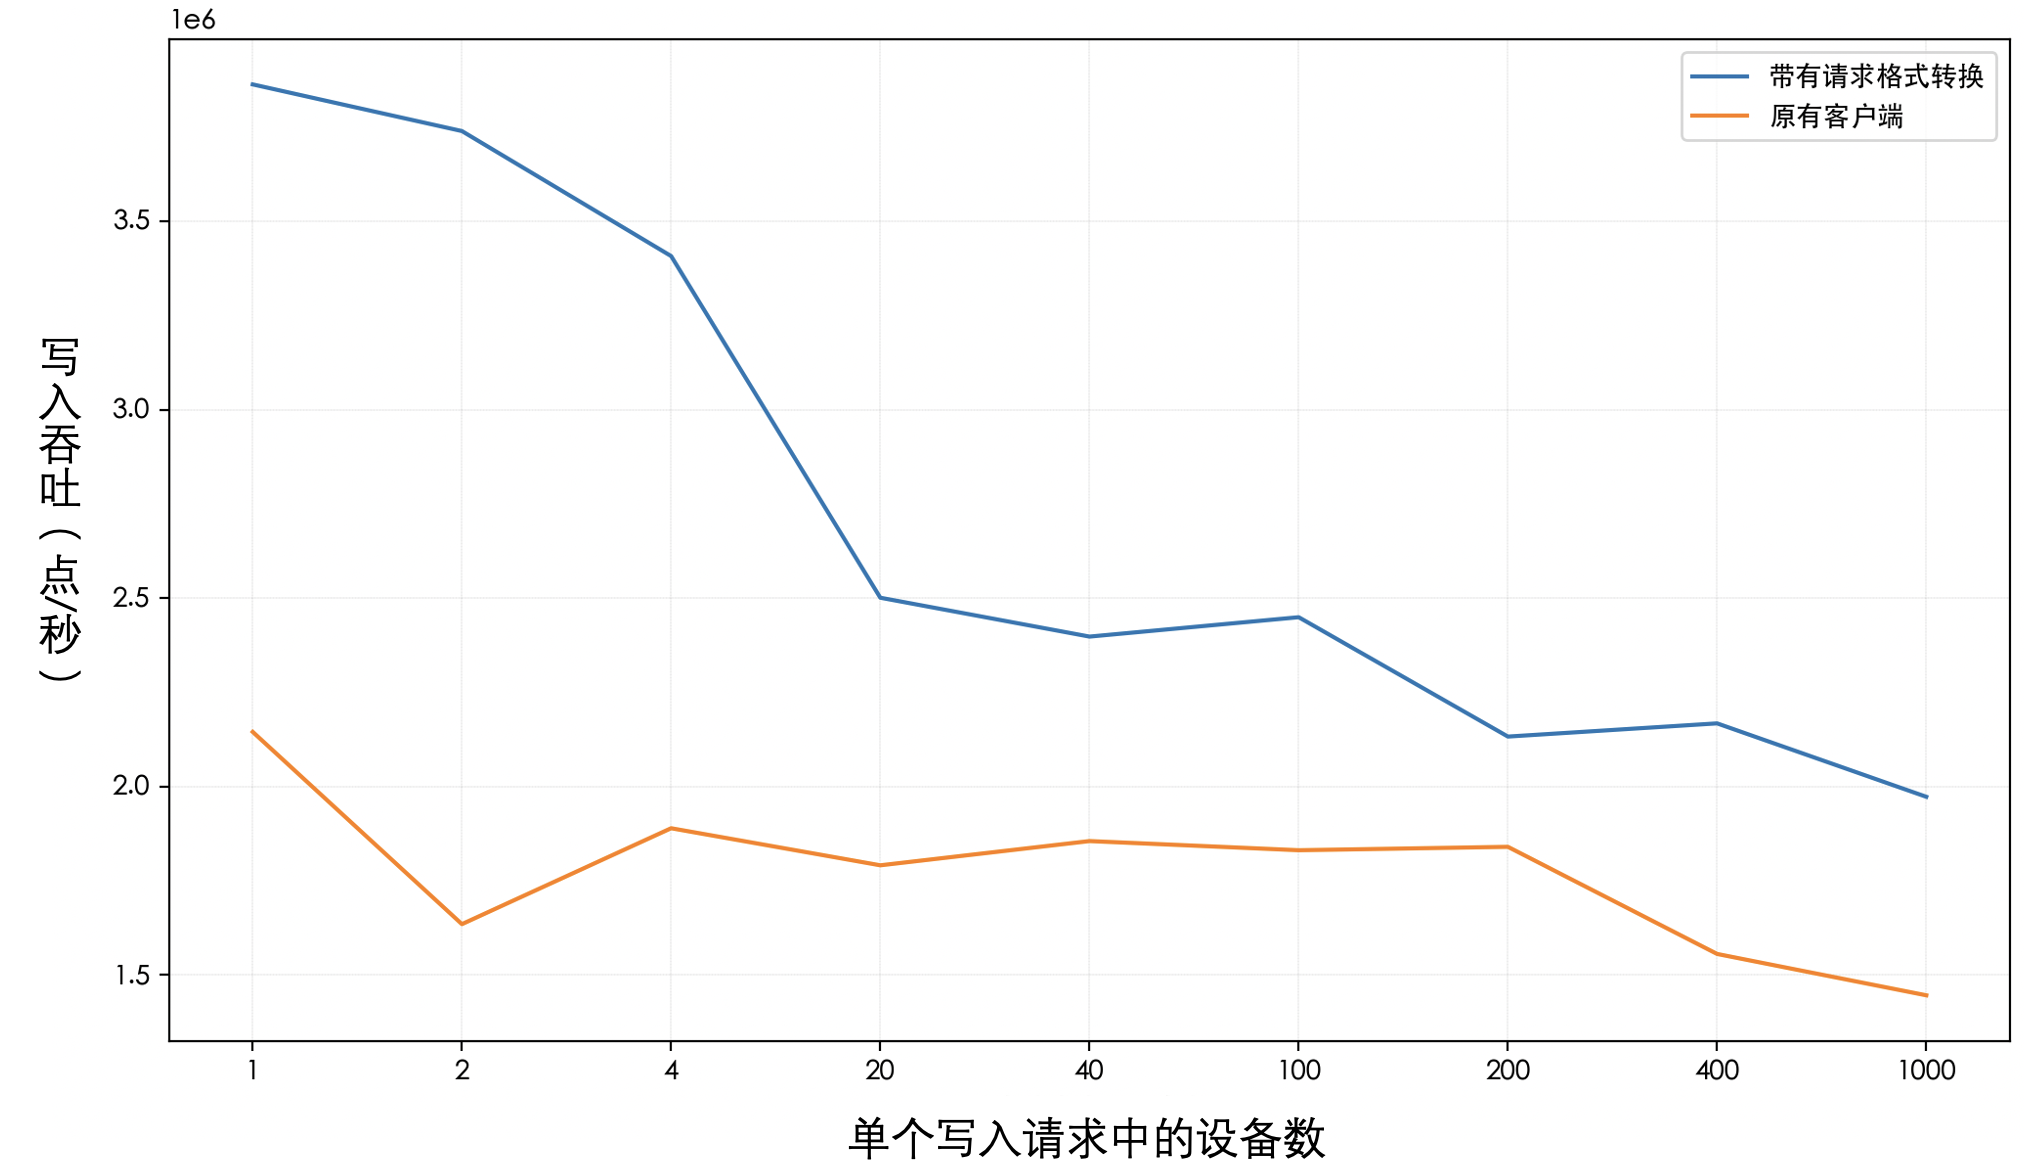
\includegraphics[width=0.9\linewidth]{Records 转换为 Tablets 性能对比.png}
  \caption{客户端请求格式转换实验吞吐量对比}
  \label{fig:records-to-tablets-performance-throughput}
\end{figure}

图 \ref{fig:records-to-tablets-performance-throughput} 展示了单一请求中设备数不同时写入吞吐的对比。客户端进行请求格式转换以后的吞吐显著高于原有客户端,当一个请求中有 2 个设备时,经过请求转换过后吞吐提高了 128\%,在测试的平均情况下提高了 54\% 的写入吞吐。

\begin{figure}
  \centering
  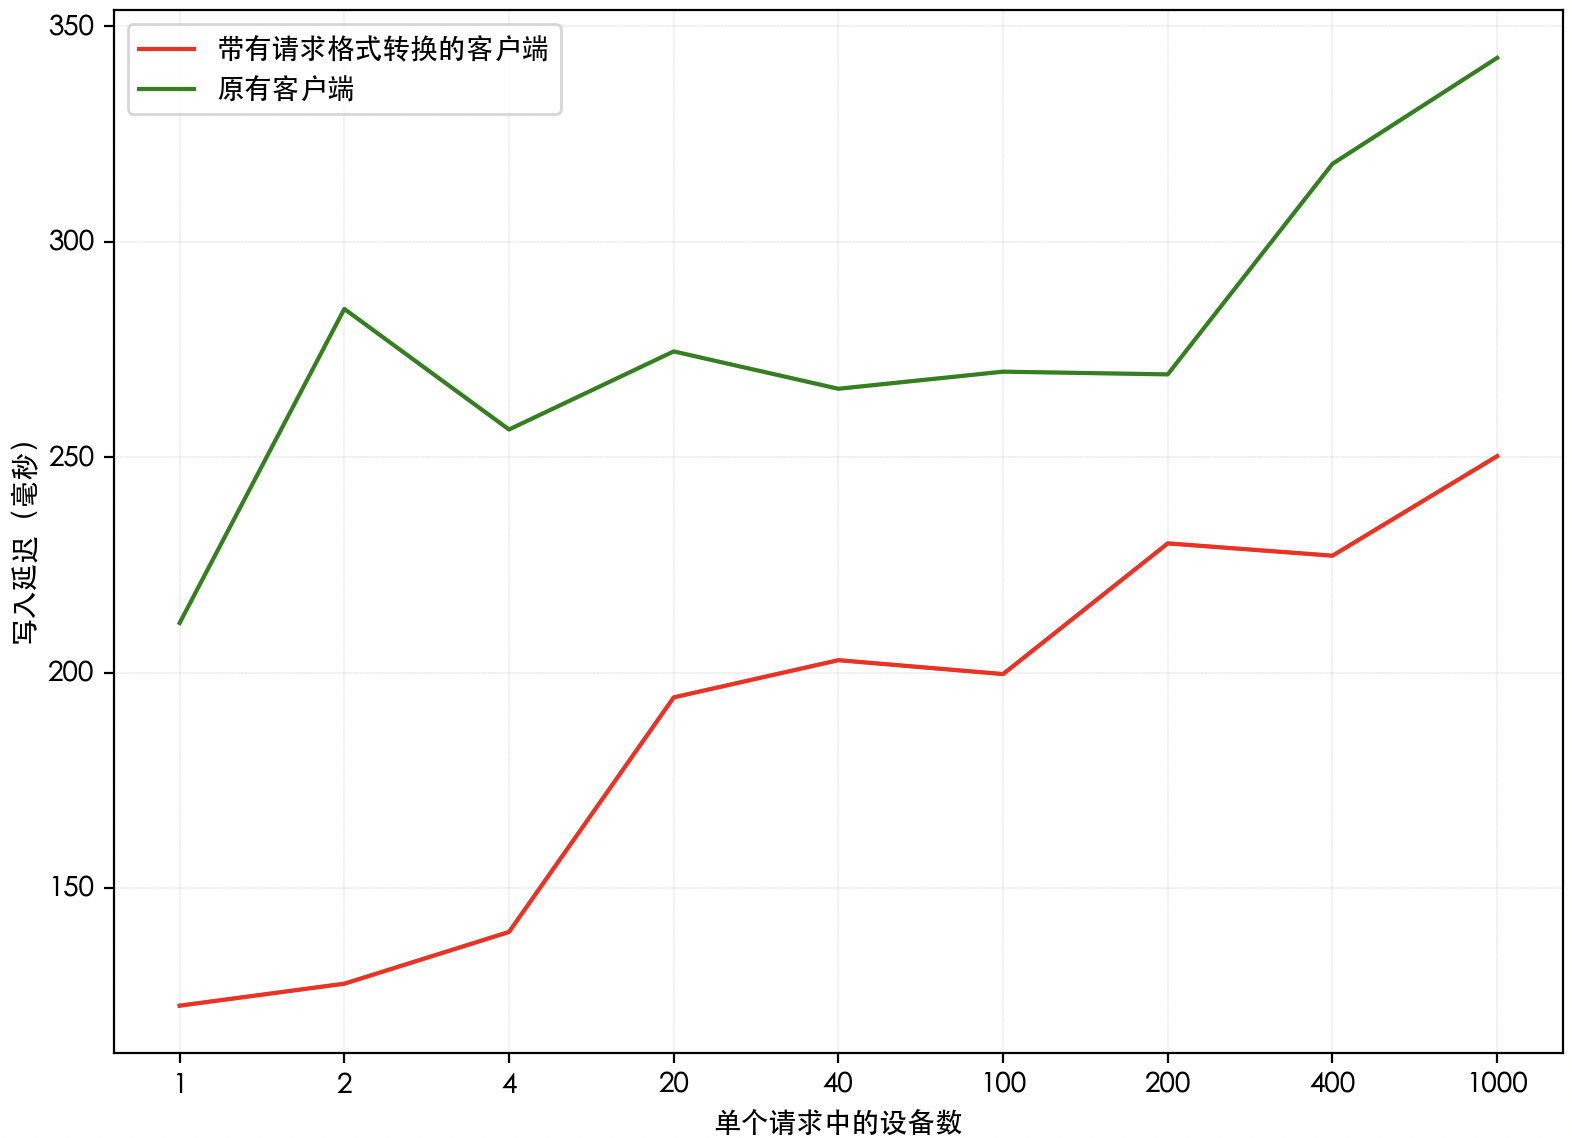
\includegraphics[width=0.8\linewidth]{Records 转 Tablets 平均延迟分布.png}
  \caption{客户端请求格式转换实验平均延迟对比}
  \label{fig:records-to-tablets-performance-avg-latency}
\end{figure}

图 \ref{fig:records-to-tablets-performance-avg-latency} 展示了单一请求中设备数不同时平均写入延迟的对比。客户端进行请求格式转换以后的延迟显著低于原有客户端,当一个请求中有 2 个设备时,经过请求转换过后平均延迟降低了 65.1\%,在测试的平均情况下写入延迟降低了 32.1\%。

\begin{figure}
  \centering
  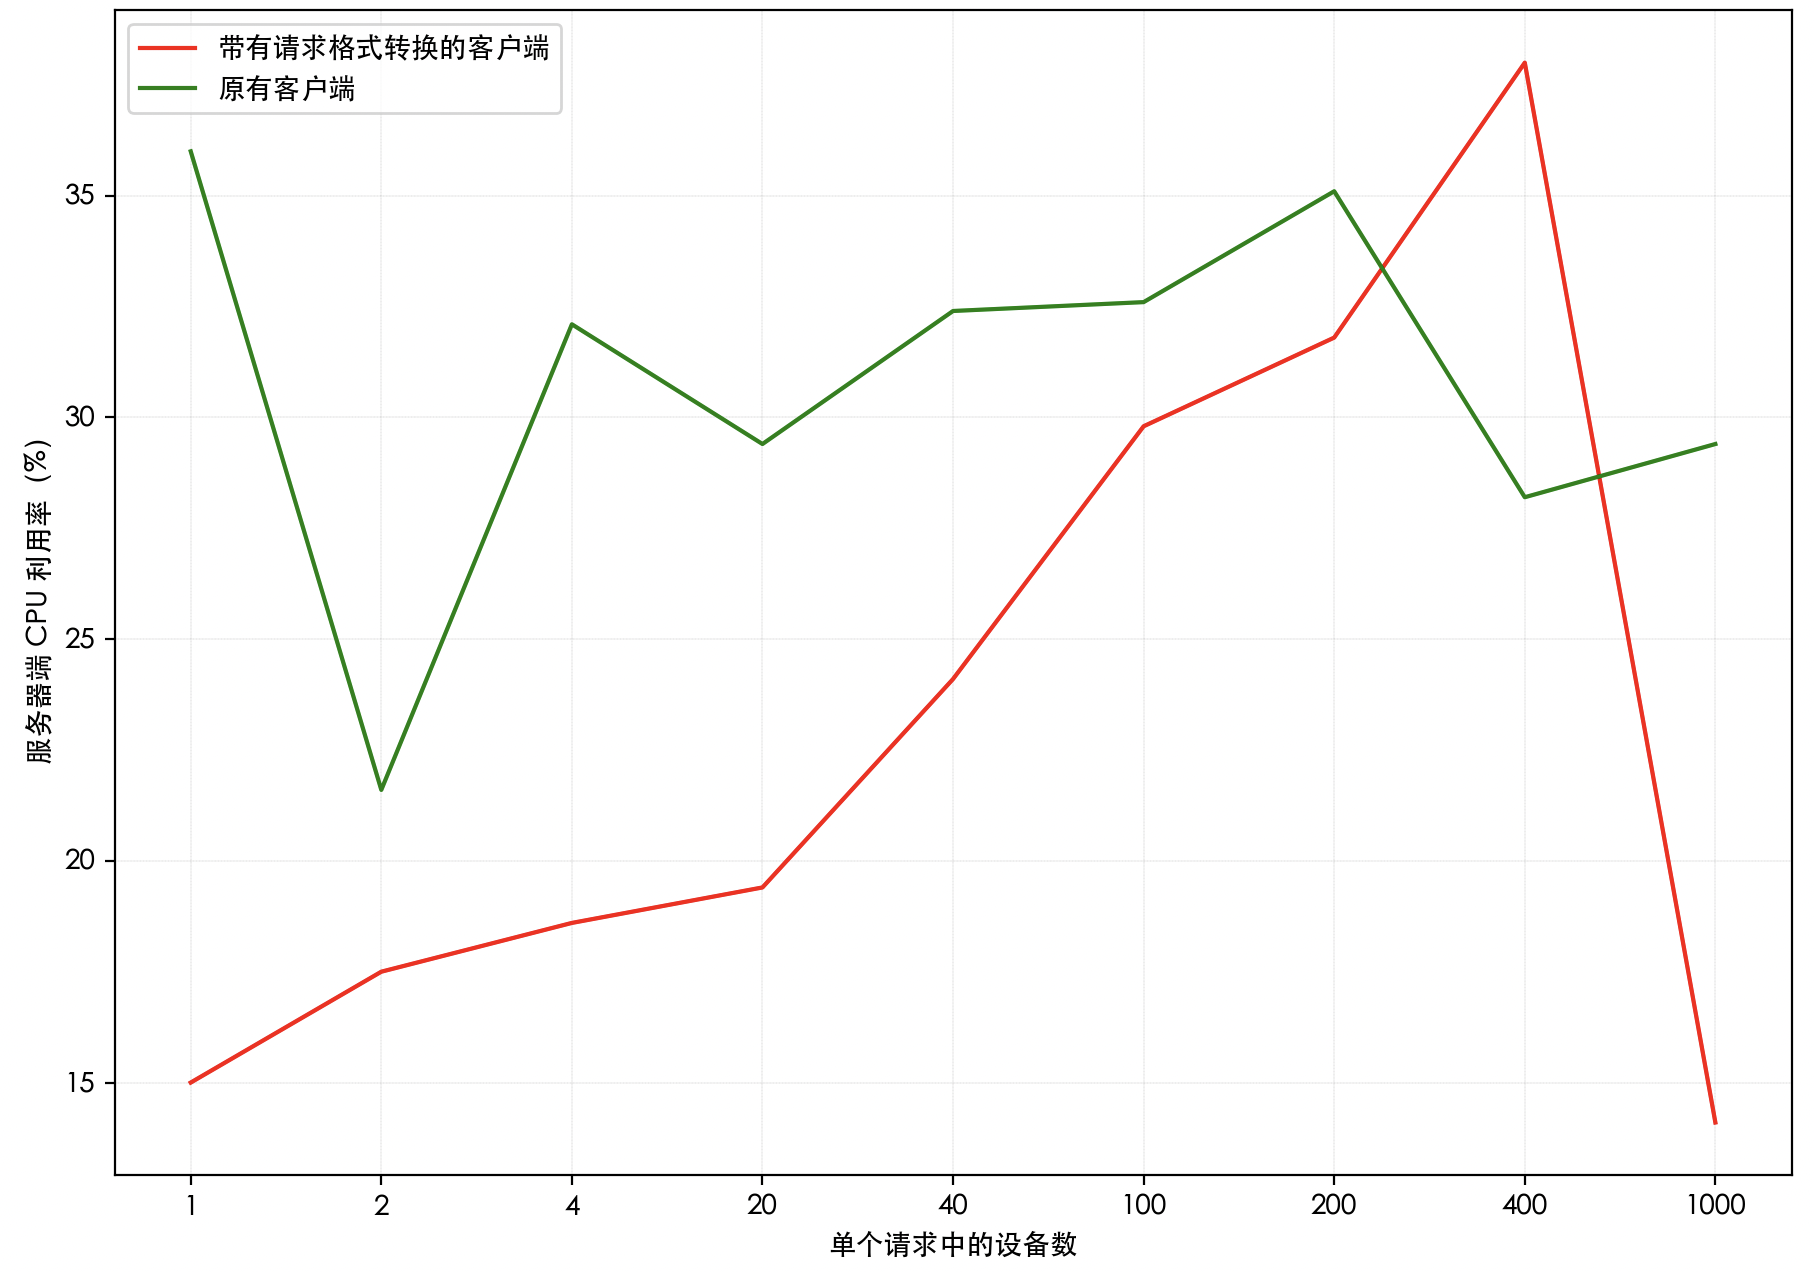
\includegraphics[width=0.8\linewidth]{Records 转 Tablets CPU 资源.png}
  \caption{客户端请求格式转换实验服务区端 CPU 资源消耗对比}
  \label{fig:records-to-tablets-performance-cpu-consuming}
\end{figure}

图 \ref{fig:records-to-tablets-performance-cpu-consuming} 展示了单一请求中设备数不同时服务端 CPU 资源消耗的对比。客户端进行请求格式转换以后的 CPU 资源消耗在大部分情况下显著低于原有客户端,当一个请求中只有 1 个设备时,经过请求转换以后服务器端的 CPU 资源消耗相对降低了 58.3\%,在平均情况下则下降了 24.8\%。但是当一个请求中的设备数为 400 个时,此时经过请求格式转换后服务器的 CPU 资源使用率反而相对上升了 34.7\%。 %TODO:探究原因

实验结果表明,当一个写入请求中每个设备平均有 2 条以上的数据时,在客户端处将它们转换为 \emph{insertTablets} 请求可以显著提高写入的吞吐,降低写入的延迟,并在大部分情况下降低服务器端的资源利用率。这是因为 \emph{insertTables} 本身是一种批量化执行的写入机制,将 \emph{insertRecords} 转换为 \emph{insertTablets} 写入可以在尽量少改动代码的情况下获取较高的收益。因此,在后续的实验中我们关注的是在不能转换为 \emph{insertTablets} 请求的场景下,即每个写入请求中每个设备都只有一条数据的情况下,如何通过其他优化手段提高写入性能。

在后续的实验中,我们先测试对存储引擎的优化所带来的性能提升,并通过实验的结果表明网络带宽已经成为了新的写入性能瓶颈,再测试列式写入序列化在这一场景下所带来的性能提升。最后,我们将所有优化点综合在一起,通过用户负载模拟程序,模拟真实用户的负载,验证所有优化点的综合效果。

\begin{table}
  \centering
  \caption{InsertRecords 写入测试 IoT Benchmark 配置}
  \begin{tabular}{ll}
    \toprule
    配置名称 & 配置值 \\
    \midrule 
    设备数 & 100000 \\
    每个设备的序列数 & 10 \\
    存储组数 & 5 \\
    写入客户端数 & 25 \\
    每个写入请求的设备数 & 1000 \\
    每个写入请求中每个设备的记录数 & 1 \\
    \bottomrule
  \end{tabular}
  \label{tabular:test-req-format-iot-benchmark-config-2}
\end{table}

表 \ref{tabular:test-req-format-iot-benchmark-config-2} 展示了后续实验中所使用的 IoT Benchmark 的配置。在这一配置下,每次写入时每个设备都只写 1 条数据,不会在客户端处被转换为 \emph{insertTablets} 请求,而是仍然会通过 \emph{insertRecords} 请求写入到 IoTDB 中。使用该配置,本工作测试了客户端路径预先校验以及内存预计算对性能的影响,表 \ref{tabular:client-offloading-performance} 展示了实验的结果。从结果中我们可以看出,客户端预先对时间序列 ID 进行校验以及预先计算内存开销后,写入的吞吐提升了 2.2\%,服务器 CPU 的占用下降了 5.2\%,由于写入数据量的提升,其他资源的占用也有所提升。

\begin{table}  
  \centering  
  \caption{客户端时间序列 ID 预校验与内存预计算性能测试结果}  
  \begin{tabular}{cccc}  
    \toprule   
    指标 & 未优化 & 客户端数据预处理 & 优化幅度 \\   
    \midrule  
    吞吐(点/秒) & 1606206 & 1642600 & +2.2\%\\  
    平均延迟(ms) & 321.00 & 313.12 & -2.4\%\\  
    P99 延迟(ms) & 1303.93 & 1769.08 & +35.6\% \\  
    服务器 CPU 消耗 & 44.4\% & 42.1\% & -5.2\%\\  
    服务器磁盘利用率 & 93.2\% & 94.2\% & +1.1\%\\  
    服务器磁盘吞吐(MB/s) & 129 & 134 & +3.9\% \\  
    网络吞吐(MB/s) & 65.4 & 70.6 & +8.0\%\\  
    \bottomrule   
  \end{tabular}  
  \label{tabular:client-offloading-performance}  
\end{table}

\section{存储引擎优化写入性能测试}
本节测试对存储的优化对性能的提升。
\subsection{存储引擎批量化写入性能测试}
存储引擎批量化写入主要包括批量化更新监控系统、批量化写入内存表、批量化更新内存缓存、批量化序列化写前日志。这四个优化点优化原理是尽可能地将可以一起被写入的数据绑定起来一起写入或操作,从而平摊写入中的一些固定开销,进而提高性能。
\begin{table}
  \centering
  \caption{批量化写入性能测试结果}
  \begin{tabular}{cccc}
    \toprule 
    指标 & 客户端数据预处理 & 批量化写入 & 优化幅度 \\ 
    \midrule  
    吞吐(点/秒) & 1642600 & 1703651 & +3.7\%\\  
    平均延迟(ms) & 313.12 & 295.73 & -5.6\%\\  
    P99 延迟(ms) & 1769.08 & 1237.56 & -30.0\% \\  
    服务器 CPU 消耗 & 42.1\% & 40.1\% & -4.8\%\\  
    服务器磁盘利用率 & 94.2\% & 92.3\% & -2.0\%\\  
    服务器磁盘吞吐(MB/s) & 134 & 130 & -3.0\% \\  
    网络吞吐(MB/s) & 70.6 & 69.1 & -2.1\%\\  
    \bottomrule
  \end{tabular}
  \label{tabular:batch-write-performance}
\end{table}

表 \ref{tabular:batch-write-performance} 展示了批量化写入对性能的提升,吞吐提升了 3.7\%,平均延迟下降了 5.6\%,在吞吐更高的情况下,服务器的 CPU 消耗量还下降了 4.8\%,磁盘的利用率下降了 2.0\%。这表明,在使用批量化写入以后,IoTDB 的执行效率变得更高了,提升了写入性能的同时降低了对部分资源的使用。

\subsection{写前日志压缩}
在表 \ref{tabular:batch-write-performance} 的实验结果中,我们发现 IoTDB 在测试过程中的磁盘利用率始终处于较高的水平,这表明磁盘的写入速度已经成为了写入性能的瓶颈。从 \ref{sec:chap3-sec3-1} 节的实验中我们发现在使用 \emph{insertRecords} 写入时,写前日志造成的 I/O 量是 TsFile 的 7 倍,这表明写前日志占用了大量的 I/O 资源。为了进一步提高写入性能,我们设计了写前日志压缩机制,将写前日志中的数据进行压缩,减少写入磁盘的数据量,从而提高写入性能。

\begin{table}
  \centering
  \caption{写前日志压缩性能测试结果}
  \begin{tabular}{cccc}
    \toprule 
    指标 & 无批量化写入 & 批量化写入 & 优化幅度 \\
    \midrule
    吞吐(点/秒) & 1703651 & 2453969 & +44.1\%\\
    平均延迟(ms) & 295.73 & 203.83 & -31.1\%\\
    P99 延迟(ms) & 1237.56 & 502.55& -59.4\% \\
    服务器 CPU 消耗 & 40.1\% & 	55.3\% & +37.9\%\\
    服务器磁盘利用率 & 92.3\% & 	66.3\% & -28.2\%\\
    服务器磁盘吞吐(MB/s) & 130 & 	74.8 & -42.5\% \\
    网络吞吐(MB/s) & 69.1 & 	99.5 & +43.9\%\\
    \bottomrule 
  \end{tabular}
  \label{tabular:wal-compression-performance}
\end{table}

表 \ref{tabular:wal-compression-performance} 展示了写前日志压缩对性能的提升,吞吐提升了 44.1\%,平均延迟下降了 31.1\%,代表极端情况的 P99 延迟则下降了 59.4\%。在吞吐提升 44.1\% 的情况下,CPU 利用里提升了 37.9\%,这表明同样 CPU 消耗的情况下写入的数据更多了。磁盘资源紧张的情况得到了显著缓解,磁盘利用率下降了 28.2\%,磁盘吞吐下降了 42.5\%,这表明磁盘已经不再是写入的瓶颈。由于写入数据量的增加,网络带宽的占用也从 69.1 MB/s 上升到了 99.5 MB/s。由于测试环境的网络理论带宽为 1000Mbps,此时的网络带宽已经接近了网络的极限,这表明网络带宽已经成为了新的写入性能瓶颈。


\section{写入请求列式序列化性能测试}
从表 \ref{tabular:wal-compression-performance} 展示的试验结果中,我们发现网络可能成为了写入的新瓶颈。为了进一步提高写入性能,我们设计了列式写入请求序列化机制,将写入请求中的数据进行列式序列化,减少写入网络的数据量,从而提高写入性能。

\begin{table}
  \centering
  \caption{列式写入请求序列化性能测试结果}
  \begin{tabular}{cp{3.5cm}p{3.5cm}c}
    \toprule 
    指标 &  无写入请求序列化 & 列式写入请求序列化 & 优化幅度 \\
    \midrule  
    吞吐(点/秒) & 2453969 & 3308927 & +34.4\%\\  
    平均延迟(ms) & 203.83 & 165.48 & -18.8\%\\  
    P99 延迟(ms) & 502.55 & 915.74 & +82.2\%\\  
    服务器 CPU 消耗 & 55.3\% & 65.5\% & +18.4\%\\  
    服务器磁盘利用率 & 66.3\% & 81.7\% & +23.2\%\\  
    服务器磁盘吞吐(MB/s) & 74.8 & 91.1 & +21.8\%\\  
    网络吞吐(MB/s) & 99.5 & 3.06 & -96.9\%\\  
    \bottomrule 
  \end{tabular}
  \label{tabular:columnar-serialization-performance}
\end{table}

表 \ref{tabular:columnar-serialization-performance} 展示了加上列式写入请求序列化的结果,吞吐提升了 34.9\%,平均延迟下降了 18.9\%。但是,由于写入请求序列化会带来编码和解编码的开销,容易让 JVM 发生更频繁的垃圾回收,所以代表极端情况的 P99 延迟反而上升了 82.2\%。在吞吐提升 34.9\% 的情况下,CPU 消耗量上升了 18.4\%,磁盘利用率上升了 23.2\%,磁盘吞吐上升了 21.8\%。网络带宽占用显著下降了 96.9\%,降为原有的 3.1\%,远低于测试环境的网络理论带宽,这表明网络带宽已经不再是写入性能的瓶颈。

\begin{table}
  \centering
  \caption{FragmentInstance 并行写入性能测试结果}
  \begin{tabular}{cp{3.5cm}p{3.5cm}c}
    \toprule 
    指标 &    FI 串行写入 &  FI 并行写入 & 优化幅度 \\
    \midrule  
    吞吐(点/秒) & 	3308927 & 3467967 & +4.8\%\\  
    平均延迟(ms) &  	165.48 & 88.3 & -6.9\%\\  
    P99 延迟(ms) & 	915.74 & 740.23 & -9.1\%\\  
    服务器 CPU 消耗 &  	65.5\% & 73.3\% & +1.9\%\\  
    服务器磁盘利用率 & 	81.7\% & 83.3\% & +1.9\%\\  
    服务器磁盘吞吐(MB/s) & 91.1 & 92.4 & +1.4\%\\  
    网络吞吐(MB/s) & 	3.06 & 3.21 & +4.9\%\\  
    \bottomrule
  \end{tabular}
  \label{tabular:fi-parallel-insert-performance}
\end{table}

表 \ref{tabular:fi-parallel-insert-performance} 展示了增加 Fragment Instance 并行插入对性能的影响。从实验结果中可以看出,Fragment Instance 并行插入以后对吞吐的影响并不显著,只增加了 $4\%$,但对延迟的降低非常显著,达到了 $47\%$。这是因为多个 Fragment Instance 可以同时写入到内存表中,使得每个 DataRegion 几乎都连续不断地在写入数据,相比于串行写入减少了写入主线程的等待时间,因此降低了延迟。但是加入 Fragment Instance 并行写入之后服务器 CPU 利用率提升的比例高于吞吐提升的比例,这意味着 CPU 写入每个数据点的开销增加了。这个现象是合理的,因为加入 Fragment Instance 并行写入以后在写入过程中引入了更多线程切换和同步的开销,导致了资源利用率的下降。但总的来说,在降低延迟方面,Fragment Instance 并行写入有着明显的效果。

最后,表 \ref{tabular:columnar-serialization-performance-vs-origin} 展示了以上三种优化措施综合起来相较于未优化之前在表 \ref{tabular:test-req-format-iot-benchmark-config-2} 负载下带来的性能提升,吞吐提升了 116\%,平均延迟下降了 73\%,P99 延迟下降了 44\%,服务器 CPU 消耗提升了 65\%,服务器磁盘利用率下降了 11\%,磁盘吞吐量减少了 28\%,网络带宽的消耗减少了 95\%。这表明通过对存储引擎和写入请求序列化的优化,IoTDB 的写入性能得到了显著提升,同时也减少了对服务器资源的消耗。

\begin{table}
  \centering
  \caption{综合性能测试结果}
  \begin{tabular}{cccc}
    \toprule 
    指标 &  未优化  & 优化后 & 优化幅度 \\
    \midrule
    吞吐(点/秒) & 1606206 & 3467967 & +115.9\% \\
    平均延迟(ms) & 321.00 & 88.3 & -72.5\% \\
    P99 延迟(ms) & 1303.93 & 740.23 & -43.2\% \\
    服务器 CPU 消耗 & 44.4\% & 73.3\% & +65.1\% \\
    服务器磁盘利用率 & 93.2\% & 83.3\% & -10.6\% \\
    服务器磁盘吞吐(MB/s) & 129 & 92.4 & -28.4\% \\
    网络吞吐(MB/s) & 65.40 & 3.21 & -95.1\% \\
\bottomrule
  \end{tabular}
  \label{tabular:columnar-serialization-performance-vs-origin}
\end{table}

\section{用户模拟负载测试}
本节使用模拟用户场景的负载对写入措施进行优化。本节首先介绍了用户负载的采样程序和模拟运行程序,然后使用中冶赛迪、四维智联和宝武集团三位用户的模拟负载对前文的优化措施进行了测试。
\subsection{负载采样程序}
目前 IoTDB 一共有超过一千家企业用户,这些用户的写入负载特征各异。例如在车联网场景中,设备数通常非常多,每个设备产生数据的频率较低;在工业监控场景中,设备数则相对较少,但每个设备产生数据的频率有可能较高。在同一个场景中,不同设备的数据产生频率、时间序列类型、时间序列数量等也可能有所不同。因此,为了更好地模拟真实用户的负载,本工作设计了一个负载采样程序,用于对用户场景特点进行采样。

负载采样程序的主要功能是通过扫描用户运行 IoTDB 所产生的 TsFile,收集时间序列的特征信息。这些信息包括:
\begin{itemize}
  \item \textbf{不同时间序列类型的比例}:IoTDB 目前支持六种类型的时间序列,分别是 INT32、INT64、FLOAT、DOUBLE、BOOLEAN 和 TEXT。不同时间序列类型的比例对于写入性能有一定影响,例如 TEXT 类型写入需要消耗更大的内存,会产生较大的写前日志,而 BOOLEAN 类型的写入则资源消耗相对较小。
  \item \textbf{时间序列数据的频率分布}:不同时间序列的数据产生频率不同,有的时间序列数据产生频率较高,有的时间序列数据产生频率较低,这是用户负载一个重要的特征。
  \item \textbf{单个设备下时间序列数量的分布}:即使在同一用户场景下,不同设备下时间序列数量也可能相差较大,负载采样程序收集每个设备下时间序列数目的分布信息,为构建负载模拟程序提供参考。
  \item \textbf{对齐时间序列与非对齐时间序列的比例}:IoTDB 目前支持两种序列类型,分别是对齐时间序列和非对齐时间序列。两种时间序列在性能上有所不同,对齐时间序列的写入性能较高,而非对齐时间序列的写入性能较低。负载采样程序收集对齐时间序列和非对齐时间序列的比例信息,为构建负载模拟程序提供参考。
  \item \textbf{时间序列的数值分布}:时间序列数据的值分布对于压缩和编码算法性能有一定的影响,负载模拟程序采集不同数据类型的值分布,为构建负载模拟程序提供参考。
\end{itemize}

\begin{figure}
  \centering
  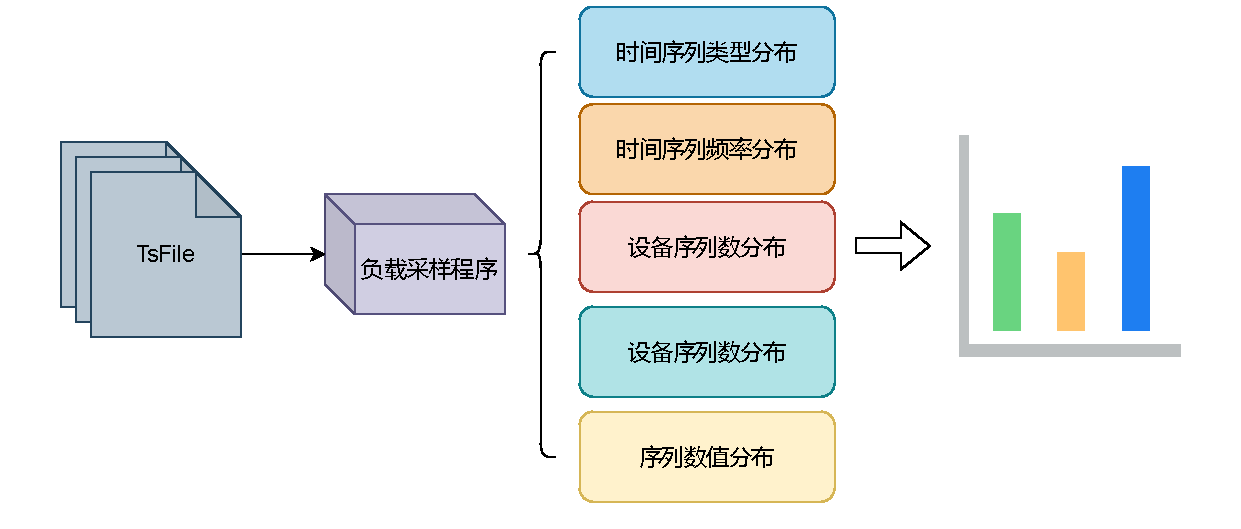
\includegraphics[width=\textwidth]{负载采样程序.pdf}
  \caption{负载采样程序架构}
  \label{fig:load-sampling-program}
\end{figure}

负载采集程序的输入是用户的 TsFile,TsFile 中的数据区分为多个数据块组(ChunkGroup),每个数据块组又分为多个数据块(Chunk)。一个数据块组就对应了一个设备,而一个数据块就对应了一个时间序列的数据。负载采样程序使用 IoTDB 所提供的 TsFileSequenceReader 顺序扫描 TsFile,通过读取每个数据块的数据类型来收集不同时间序列类型的比例,通过读取一个数据块中最大时间点与最小时间点的时间差除以数据点的数目来收集时间序列的频率分布,通过统计每个数据块组下数据块的数目来收集单个设备下时间序列数量的分布,通过读取每个数据块组的类型(对齐或非对齐)来收集对齐时间序列与非对齐时间序列的比例,通过读取每个数据块的数据值来收集不同类型时间序列的数值分布。最后,负载模拟程序将采集到的信息以直方图的形式输出为一个文件,供负载模拟程序使用。

\subsection{负载模拟程序}
图 \ref{fig:load-simulation-program} 展示了模拟负载程序的架构,模拟负载程序接收两个输入,一个是负载采样程序输出的直方图文件,另一个是负载的总设备数。模拟负载程序的运行主要分为两步,第一步是根据直方图和总设备数生成测试的时间序列和设备元数据,第二步则是根据时间序列和设备元数据模拟用户的写入请求。

\begin{figure}
  \centering
  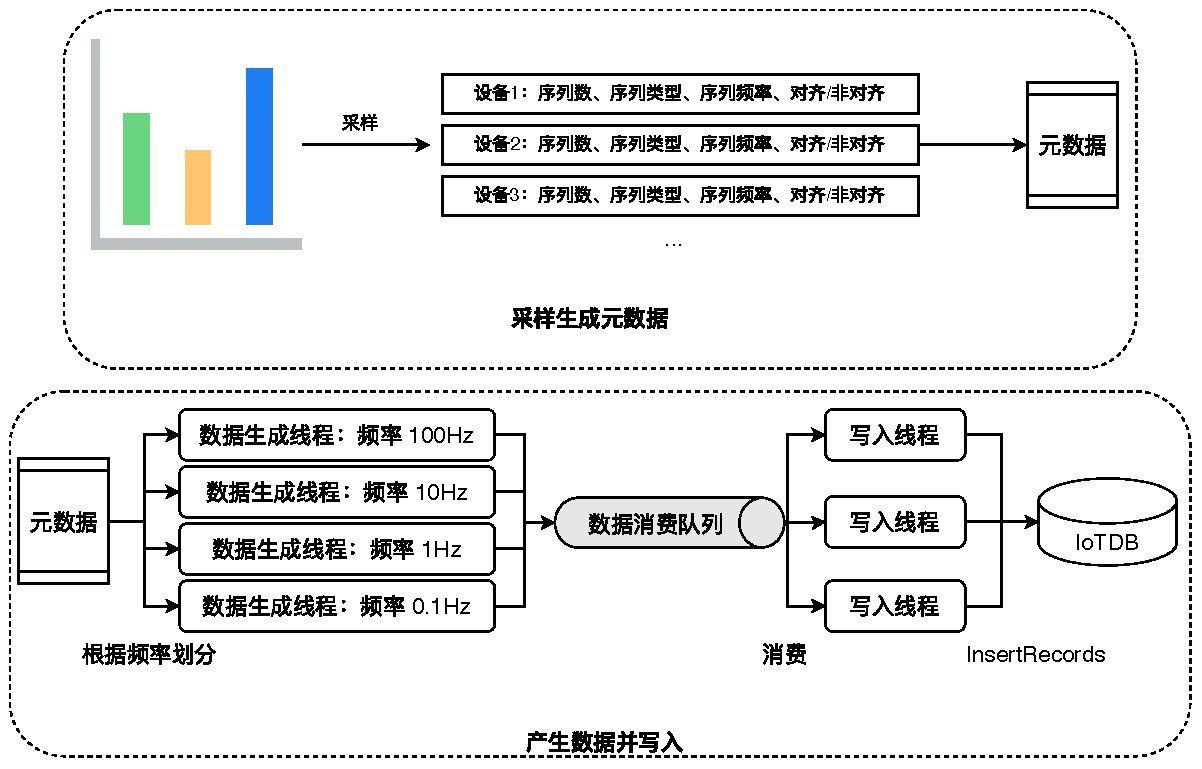
\includegraphics[width=\linewidth]{模拟负载运行程序.pdf}
  \caption{负载模拟程序架构}
  \label{fig:load-simulation-program}
\end{figure}

模拟负载程序运行的第一步是生成测试所需的元数据,这里的元数据既包含了在 IoTDB 中注册时间序列所需的信息,如每个设备下的序列数、序列名称、序列类型,也包含了模拟程序产生数据点所需的信息,如序列的频率、序列的值分布。这些数据的产生通过按照直方图中的分布随机采样得到。一个设备首先会先根据对每个设备下时间序列数的分布进行随机采样,得到本设备的序列数,然后再对频率直方图采样得到本设备下所有时间序列的数据生成频率。然后对于本设备下的每个时间序列,再采样得到其数据类型、值分布等。最后,模拟负载程序一方面将时间序列的元数据注册到 IoTDB 中,另一方面也会将这些信息保存在内存中,用于后续模拟数据的生成和写入。

模拟负载程序运行的第二步是模拟用户的写入请求。模拟负载程序首先会将第一步中生成的设备按照产生数据的频率进行划分,相同频率的设备被归类到一起。然后,具有相同频率的设备会被放到同一个数据生成线程中,这个线程会按照这批设备的频率周期性地按照每个设备的值分布产生数据。如果某一个频率的设备数过多,使用一个线程有可能导致无法按照规定的周期产生数据。例如,如果有大量 100 Hz 的设备,理论上每个设备每隔 10 ms 就要产生一批数据,但是一个线程有可能无法在 10 ms 内产生所有设备的数据,这就会导致最终设备生成数据的频率小于 100 Hz。为了避免这样的情况,每个线程最多负责 5000 个设备的数据生成。这样,即使设备数较多,也可以保证每个设备的数据生成频率不会受到影响。每个数据生成线程会将周期性产生的数据放入一个有限大小的内存并发队列中等待写入线程的消费,如果队列满了就会放弃将数据放入队列,并通过日志记录这种情况。写入队列会不断地从队列中取出数据并在本地缓存生成一个写入请求,如果写入请求的记录行数超过 2000 条或者该写入请求中最旧的数据点的时间戳距离当前时间超过 10 秒,就会将该写入请求通过 \emph{insertRecords} 接口写入到 IoTDB 中。写入线程的数量可以进行调节,以模拟不同的场景。在这样的设计下,模拟负载程序可以容忍 IoTDB 一定的写入延迟波动,从而更好地模拟真实用户的负载。
\subsection{测试负载描述}
利用负载采样程序和负载模拟程序,我们分析了中冶赛迪、四维智联、宝武钢铁集团三家用户的负载,构建了这三家用户的模拟负载程序。
\begin{figure}
  \centering
  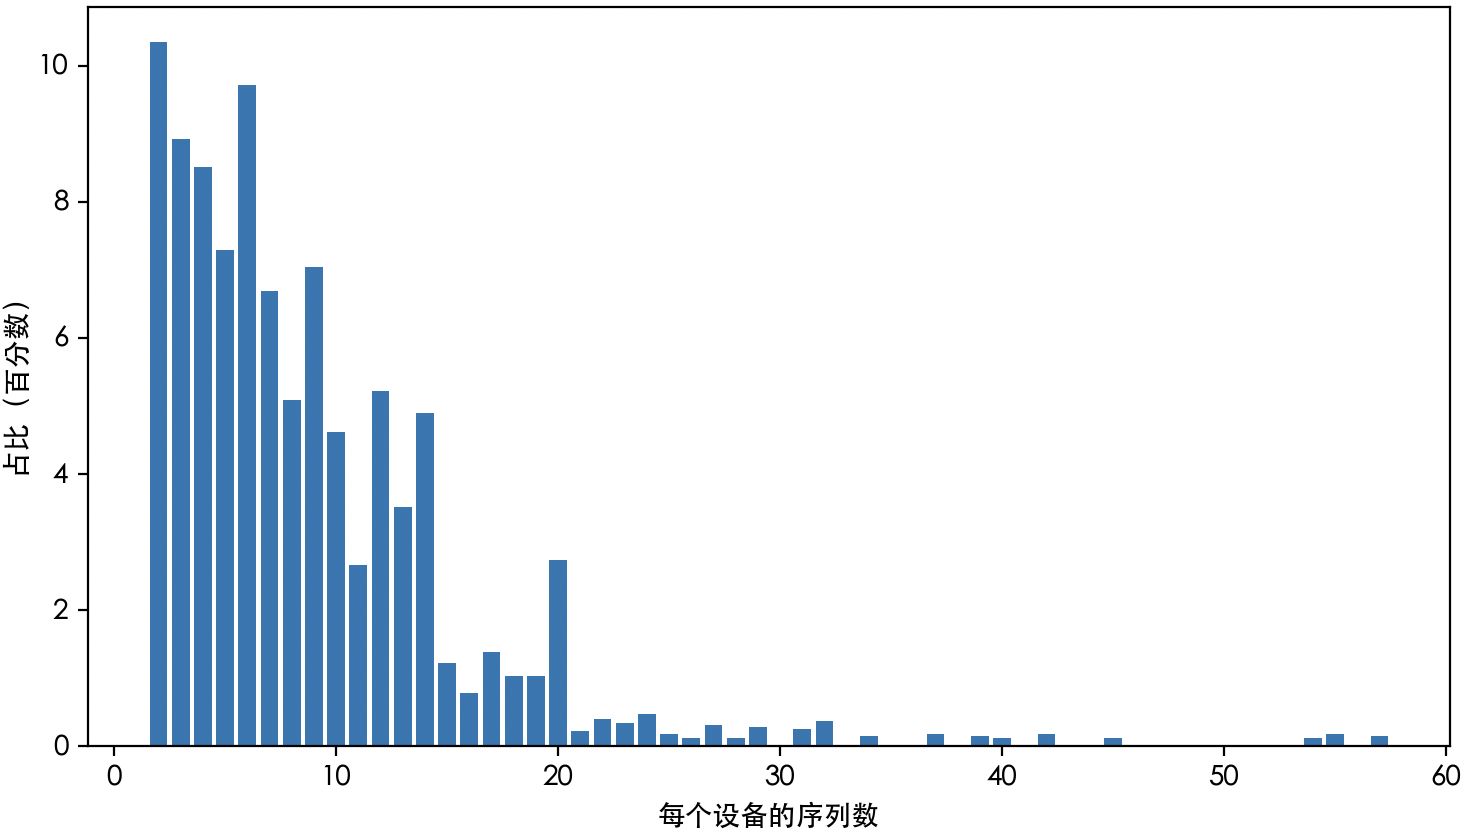
\includegraphics[width=0.7\linewidth]{中冶赛迪-镔鑫项目设备序列数分布图.png}
  \caption{中冶赛迪-镔鑫项目设备序列数分布图}
  \label{fig:zysd-bx-device-measurement-count}
\end{figure}

\begin{figure}
  \centering
  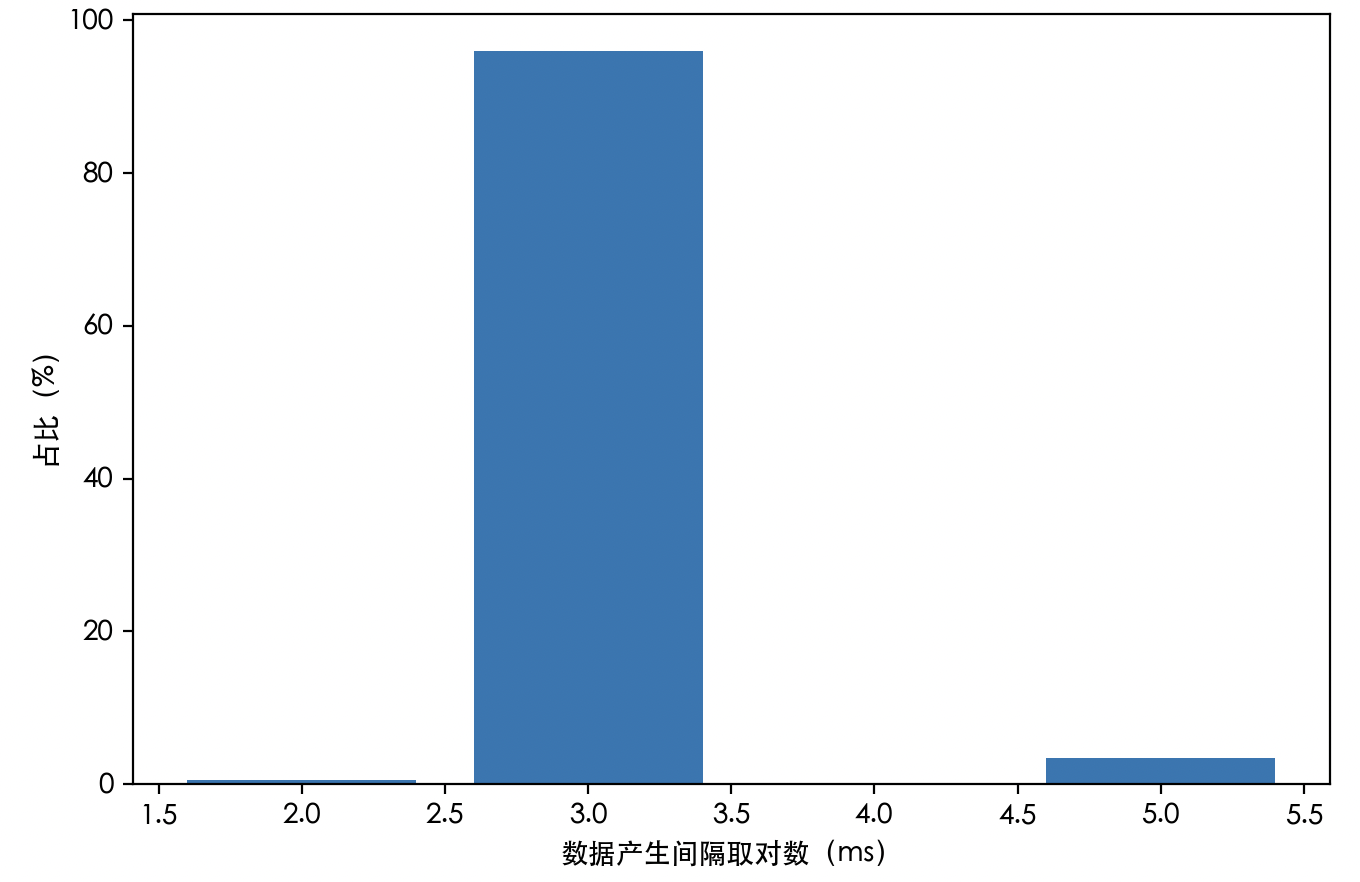
\includegraphics[width=0.7\linewidth]{中冶赛迪镔鑫项目频率分布.png}
  \caption{中冶赛迪-镔鑫项目时间序列频率分布图}
  \label{fig:zysd-bx-freq-distribution}
\end{figure}

中冶赛迪模拟负载包含了 20 万个设备与 353.2 万条时间序列,其设备序列数分布如图 \ref{fig:zysd-bx-device-measurement-count} 所示,时间序列的频率分布如图 \ref{fig:zysd-bx-freq-distribution} 所示。中冶赛迪镔鑫负载中大部分序列都是 1 秒产生一个时间点,少量序列几百秒才产生一次数据,极少数序列每隔一百毫秒就会产生一个数据点。每个设备的时间序列数量主要为 2-15 个。根据时间序列数与序列的频率计算,理想情况下数据库需要写入 3391316 个数据点。
\begin{figure}
  \centering
  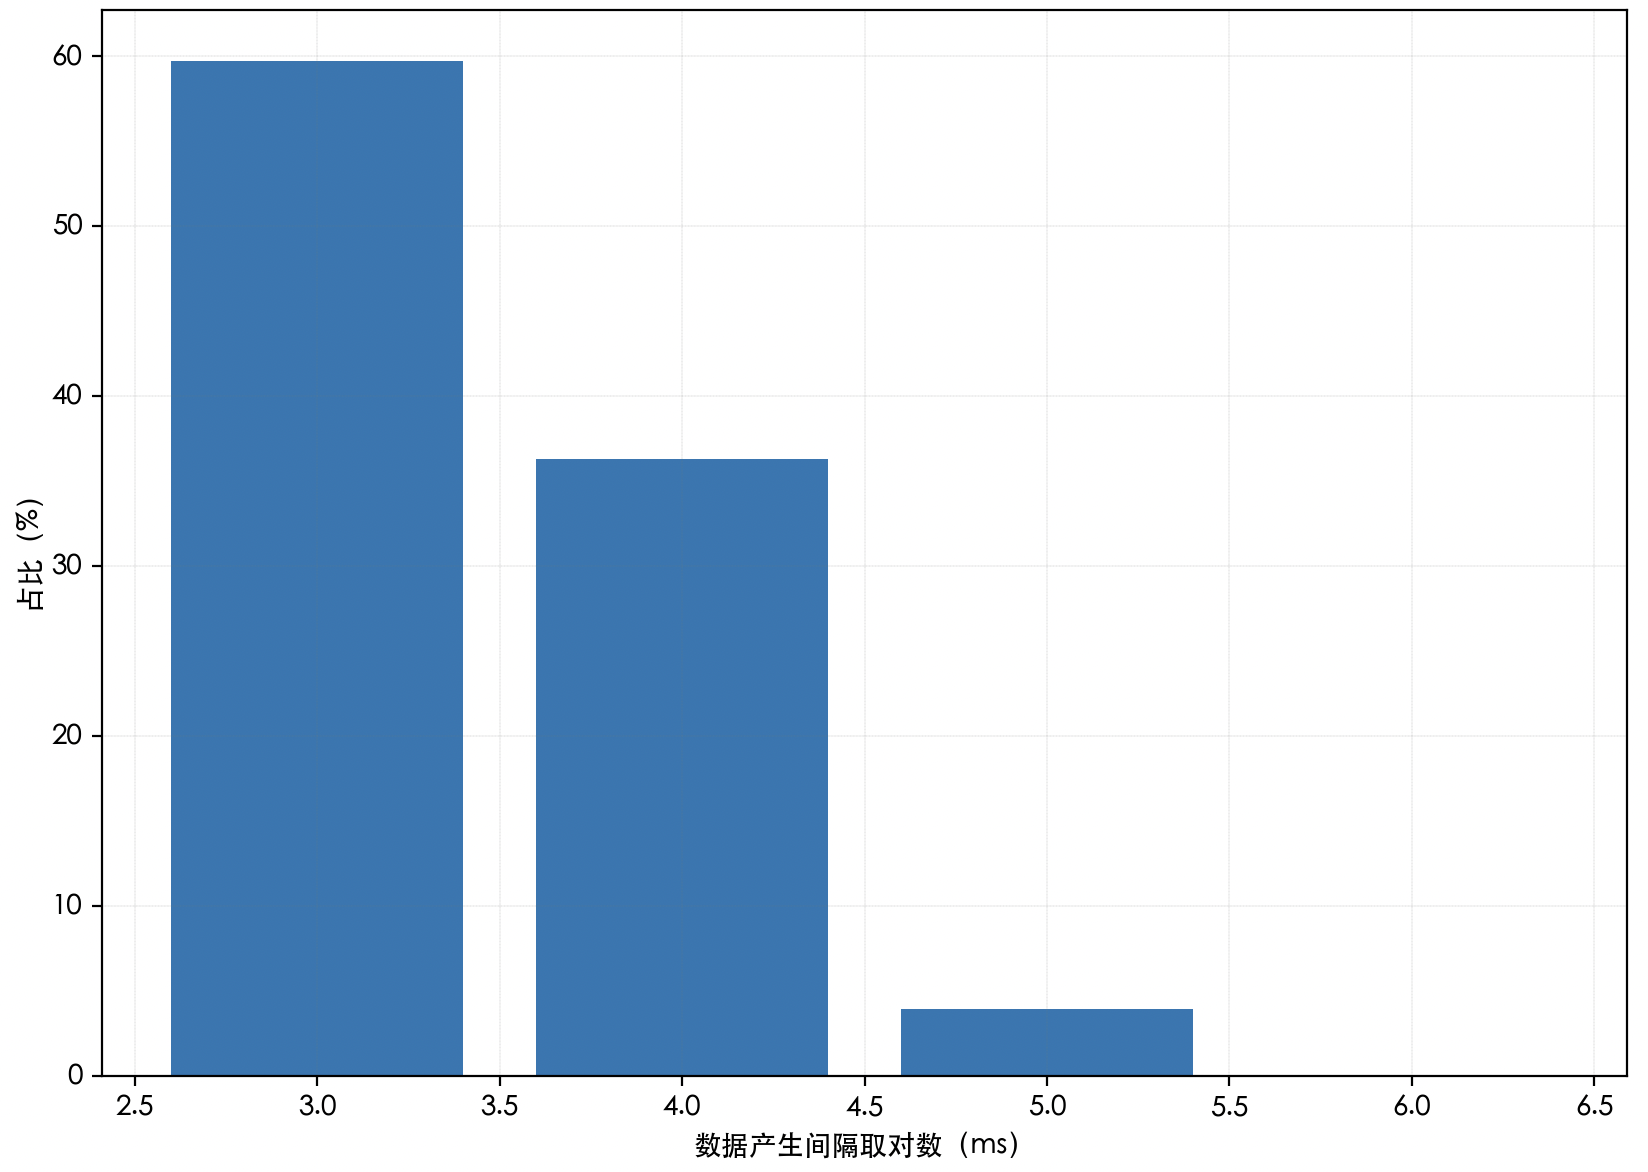
\includegraphics[width=0.7\linewidth]{四维智联时间序列频率分布.png}
  \caption{四维智联时间序列频率分布图}
  \label{fig:swzl-freq-distribution}
\end{figure}

四维智联的负载每个设备下都有 27 条时间序列,其频率分布如图 \ref{fig:swzl-freq-distribution} 所示,其中超过一半的序列每隔 1 秒钟就会产生一个数据点,大约 35\% 的序列每隔 10 秒才会产生一次数据点,剩下的序列每隔 100 秒才会产生一次数据点。其包含了 25 万个设备和 675 万条时间序列,按照数据产生的频率计算,每秒钟应该写入 1110330 个数据点。

\begin{figure}
  \centering
  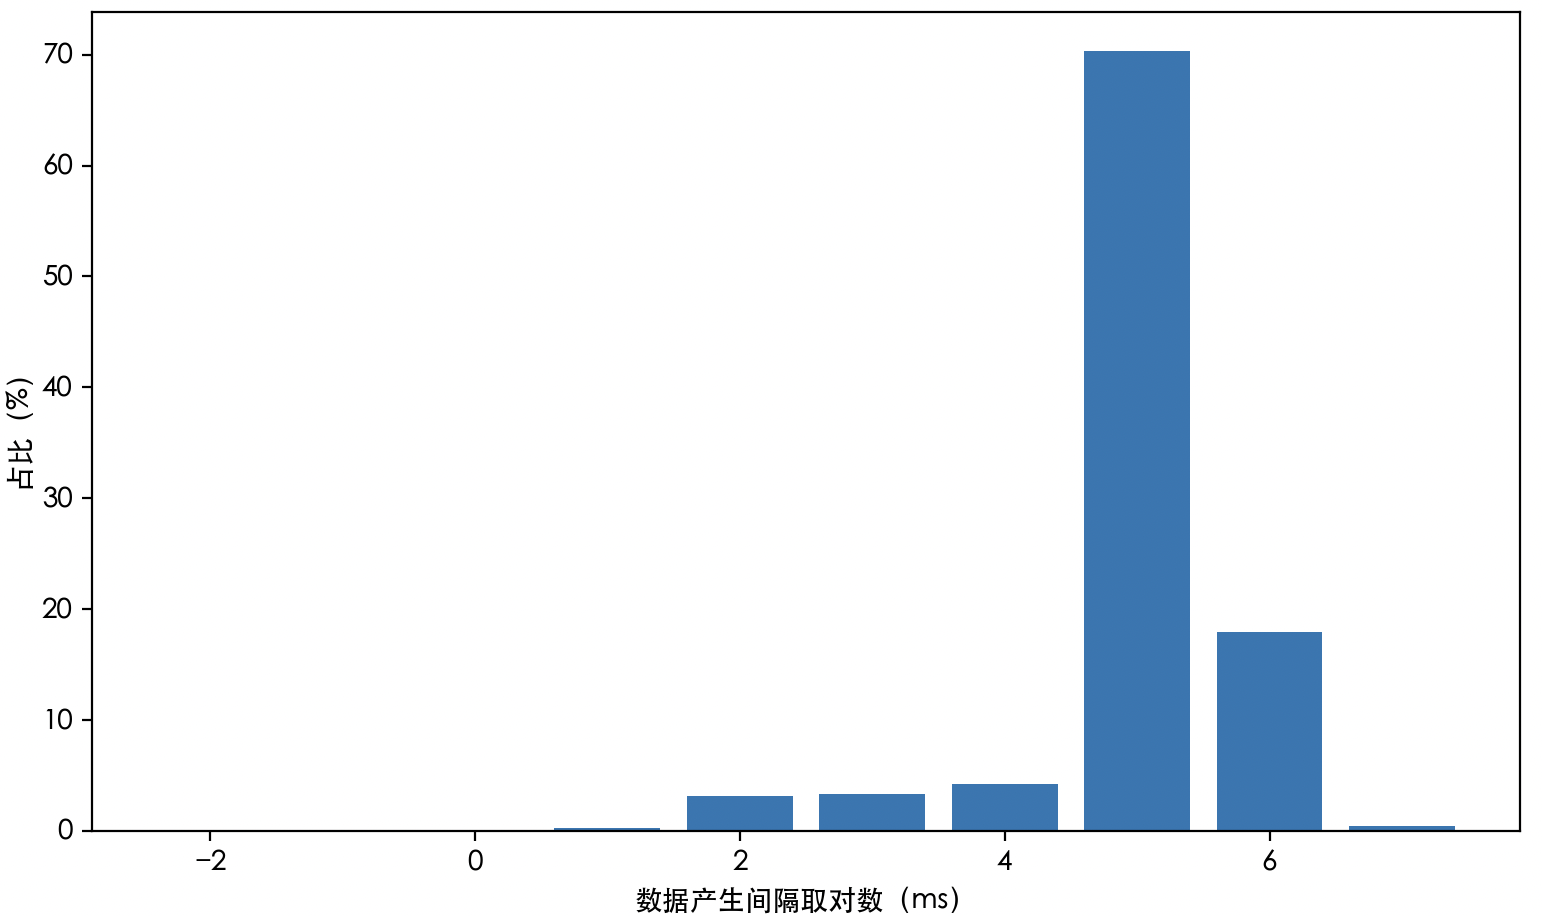
\includegraphics[width=0.5\linewidth]{宝武集团时间序列频率分布.png}
  \caption{宝武集团时间序列频率分布图}
  \label{fig:bw-freq-distribution}
\end{figure}

宝武集团的负载特征如图 \ref{fig:bw-freq-distribution} 和图 \ref{fig:bw-device-measurement-count} 所示,其每个设备的序列数大部分为 1 个或 3 个,时间序列由少量极高频(每隔 $10^{-2}$ 毫秒就产生一个数据点)和大量低频(每隔 100 秒才产生一个数据点)以及一些中频(每隔几秒或几十秒产生一个数据点)组成。其包含 25 万个设备和 267516 条时间序列,根据序列数量和序列的频率计算,理想情况下每秒钟应该写入 1410360 个数据点。

\begin{figure}
  \centering
  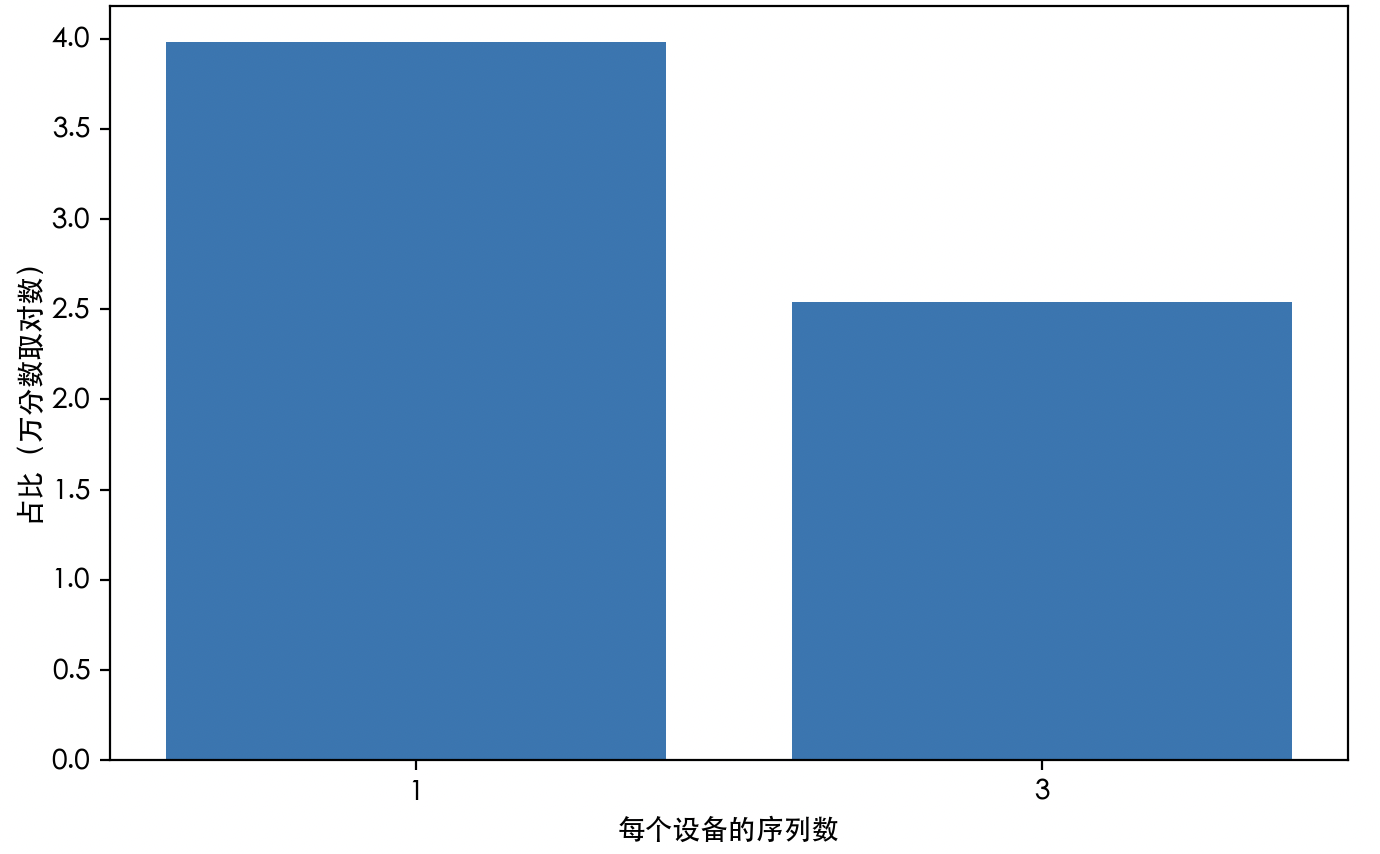
\includegraphics[width=0.7\linewidth]{宝武集团设备序列数分布.png}
  \caption{宝武集团设备序列数分布图}
  \label{fig:bw-device-measurement-count}
\end{figure}

以上三个用户场景构成了模拟负载的集合,我们将使用这些负载来测试前文的优化措施对 IoTDB 写入性能的提升。 
\subsection{测试结果}

\begin{table}
  \centering
  \caption{中冶赛迪-镔鑫项目模拟测试结果}
  \begin{tabular}{cccc}
    \toprule 
    指标 &  未优化  & 优化后 & 优化幅度 \\
    \midrule
    吞吐(点/秒) & 3392313 & 3391449 & -0.1\%\\
    平均延迟(ms) & 226 & 	117 & -48.2\%\\
    服务器 CPU 消耗 & 61.9\% & 	49.0\% & -20.8\%\\
    服务器磁盘利用率 & 60.8\% & 	33.3\% & -45.2\%\\
    服务器磁盘吞吐(MB/s) & 90.9 & 32.2 & -64.6\% \\
    网络吞吐(MB/s) & 46.4 & 38.1 & -17.9\%\\
    \bottomrule
  \end{tabular}
  \label{tabular:zysd-test-result}
\end{table}
表 \ref{tabular:zysd-test-result} 展示了中冶赛迪-镔鑫模拟负载下 IoTDB 优化前后的性能差异。优化前后的 IoTDB 都可以满足该负载的写入需求,但优化后的 IoTDB 在满足该负载写入请求的情况下平均写入延迟下降了 48\%,CPU、磁盘和网络资源的消耗分别减少了 21\%、46\% 和 18\%。这说明优化后的 IoTDB 在这一场景下处理写入请求的效率更高,因此消耗的资源更少。


\begin{table}
  \centering
  \caption{四维智联负载模拟测试结果}
  \begin{tabular}{cccc}
    \toprule 
    指标 &  未优化  & 优化后 & 优化幅度 \\
    \midrule  
    吞吐(点/秒) & 1108262 & 1112883 & +0.4\%\\  
    平均延迟(ms) & 242 & 165 & -31.8\%\\  
    服务器 CPU 消耗 & 17.4\% & 16.5\% & -5.2\%\\  
    服务器磁盘利用率 & 25.8\% & 16.0\% & -38.0\%\\  
    服务器磁盘吞吐(MB/s) & 37.2 & 17.0 & -54.3\% \\  
    网络吞吐(MB/s) & 16.7 & 5.34 & -68.0\%\\  
    \bottomrule 
  \end{tabular}
  \label{tabular:swzl-test-result}
\end{table}
表 \ref{tabular:swzl-test-result} 展示了在四维智联模拟负载下 IoTDB 优化前后的性能对比,由于四维智联负载压力并不高,优化前后的 IoTDB 都可以满足这个负载的写入需求,但优化优化后 IoTDB 的写入延迟低了 31.8\%。但是在资源占用上,优化后的 IoTDB 的 CPU、磁盘和网络资源消耗的比优化前少了 5.2\%、38.0\%、68.0\%,这表明在完成相同写入的情况下优化后的 IoTDB 资源占用更少,用户在配置服务器时可以选择较低的配置,节约成本。

\begin{table}
  \centering
  \caption{宝武负载模拟测试结果}
  \begin{tabular}{cccc}
    \toprule 
    指标 &  未优化  & 优化后 & 优化幅度 \\
    \midrule
    吞吐(点/秒) & 772071 & 1410360 & +82.7\%\\  
    平均延迟(ms) & 63.4 & 118 & +86.1\%\\  
    服务器 CPU 消耗 & 69.0\% & 35.9\% & -48.0\%\\  
    服务器磁盘利用率 & 40.9\% & 16.6\% & -60.1\%\\  
    服务器磁盘吞吐(MB/s) & 55.2 & 8.07 & -85.3\% \\  
    网络吞吐(MB/s) & 35.4 & 17.3 & -51.1\%\\ 
    \bottomrule
  \end{tabular}
  \label{tabular:bw-performance}
\end{table}
表 \ref{tabular:bw-performance} 展示了在宝武模拟负载的场景下,IoTDB 在优化前后的性能表现。在优化之前,IoTDB 未能满足宝武模拟负载的写入需求,而在优化之后 IoTDB 则可以满足其写入需求。优化后的 IoTDB 写入吞吐是优化前的 1.81 倍,服务器的 CPU、磁盘和网络资源消耗的比优化前少了 48\%、60\% 和 51\%。在这个场景下,一个写入请求中的每一行记录都只有 1 个或 3 个数据点,因此相对而言写入内存表等开销较低。但是,其他部分的开销降低了以后就意味着写入线程会频繁地向写前日志项队列中放入写前日志项,当写前日志项队列满了以后就会阻塞写入线程,造成新的瓶颈。在未优化之前,IoTDB 每一行记录都会产生一个写前日志项,在优化之后一个 FragmentInstance 才会产生一个写前日志项,日志项的数量大大降低,因此可以解除写前日志项队列所造成的瓶颈。

综合以上模拟用户场景的测试结果,在中冶赛迪-镔鑫模拟负载和四维智联模拟负载中,优化前后的 IoTDB 都可以满足负载的写入需求,但优化后的 IoTDB 占用的资源更少,写入效率更高,在对应的真实场景中可以帮助用户节约机器资源,降低生产成本;在宝武集团的模拟负载中,未优化的 IoTDB 无法满足该场景的写入需求,而优化后的 IoTDB 则可以很好地满足需求,并且占用的资源也更少。这表明,经过本工作优化后 IoTDB 的 \emph{insertRecords} 写入机制性能和效率都得到了提升,实现了本工作的目标。
\section{本章小结}
本章首先使用 IoT Benchmark 测试了当一个写入请求中每个设备有多条记录的情况下将 \emph{insertRecords} 转换为 \emph{insertTablets} 所带来的性能提升,然后测试了每个设备都只有一行记录的情况下无法转换为 \emph{insertTablets} 时,写前日志压缩、批量化写入、写入请求列式序列化、Fragment Instance 并行写入等优化点对于写入性能的提升。最后,本章介绍了本工作开发的用户负载采样程序和模拟运行程序,验证了在中冶赛迪、四维智联和宝武集团三家用户的模拟负载下本工作的优化措施对 IoTDB 写入性能的提升。